\documentclass{article}
\usepackage[utf8]{inputenc}
\usepackage{../../utils/personalmacros}

\title{Algorithmics Exercise 3}
\author{Konstantin Mark}
\date{December 2022}

\begin{document}

\maketitle


\listoftheorems[ignoreall,show={exercise}]

\newpage

%done
\begin{exercise}[Determining Treewitdth]
    Determine the treewidth of the graph depicted below by proving matching upper and lower bounds.
\end{exercise}
\begin{solving}
    By contracting the edges $(k, k+5), k = 1, \dots, 5$ we get the fully connected graph with $5$ vertices. Therefore, the treewidth is at least $4$.
     \begin{equation*}
         \begin{tikzcd}[column sep=tiny, row sep =small]
             &&& \bullet \\
	&&& \bullet \\
	\bullet & \bullet &&&& \bullet & \bullet \\
	\\
	&& \bullet && \bullet \\
	& \bullet &&&& \bullet
	\arrow[no head, from=2-4, to=5-5]
	\arrow[no head, from=2-4, to=5-3]
	\arrow[no head, from=3-2, to=3-6]
	\arrow[no head, from=3-2, to=5-5]
	\arrow[no head, from=3-6, to=5-3]
	\arrow[no head, from=5-3, to=6-2]
	\arrow[no head, from=3-1, to=3-2]
	\arrow[no head, from=3-6, to=3-7]
	\arrow[no head, from=5-5, to=6-6]
	\arrow[no head, from=2-4, to=1-4]
	\arrow[no head, from=1-4, to=3-1]
	\arrow[no head, from=1-4, to=3-7]
	\arrow[no head, from=3-7, to=6-6]
	\arrow[no head, from=6-2, to=6-6]
	\arrow[no head, from=3-1, to=6-2]
         \end{tikzcd} \to 
         \begin{tikzcd}[column sep=tiny, row sep =small]
	&& \bullet \\
	&& \bullet \\
	\bullet &&&& \bullet & \bullet \\
	\\
	& \bullet && \bullet \\
	\bullet &&&& \bullet
	\arrow[no head, from=2-3, to=5-4]
	\arrow[no head, from=2-3, to=5-2]
	\arrow[no head, from=3-1, to=3-5]
	\arrow[no head, from=3-1, to=5-4]
	\arrow[no head, from=3-5, to=5-2]
	\arrow[no head, from=5-2, to=6-1]
	\arrow[no head, from=3-5, to=3-6]
	\arrow[no head, from=5-4, to=6-5]
	\arrow[no head, from=2-3, to=1-3]
	\arrow[no head, from=1-3, to=3-6]
	\arrow[no head, from=3-6, to=6-5]
	\arrow[no head, from=6-1, to=6-5]
	\arrow[no head, from=1-3, to=3-1]
	\arrow[no head, from=3-1, to=6-1]
\end{tikzcd} \to 
     \end{equation*}
    \begin{equation*}
        \begin{tikzcd}[column sep=tiny, row sep =small]
	&& \bullet \\
	&& \bullet \\
	\bullet &&&& \bullet & \bullet \\
	\\
	& \bullet && \bullet \\
	&&&& \bullet
	\arrow[no head, from=2-3, to=5-4]
	\arrow[no head, from=2-3, to=5-2]
	\arrow[no head, from=3-1, to=3-5]
	\arrow[no head, from=3-1, to=5-4]
	\arrow[no head, from=3-5, to=5-2]
	\arrow[no head, from=3-5, to=3-6]
	\arrow[no head, from=5-4, to=6-5]
	\arrow[no head, from=2-3, to=1-3]
	\arrow[no head, from=1-3, to=3-6]
	\arrow[no head, from=3-6, to=6-5]
	\arrow[no head, from=1-3, to=3-1]
	\arrow[no head, from=3-1, to=5-2]
	\arrow[no head, from=5-2, to=6-5]
\end{tikzcd} \to 
 \begin{tikzcd}[column sep=tiny, row sep =small]
	&& \bullet \\
	&& \bullet \\
	\bullet &&&& \bullet & \bullet \\
	\\
	& \bullet && \bullet
	\arrow[no head, from=2-3, to=5-4]
	\arrow[no head, from=2-3, to=5-2]
	\arrow[no head, from=3-1, to=3-5]
	\arrow[no head, from=3-1, to=5-4]
	\arrow[no head, from=3-5, to=5-2]
	\arrow[no head, from=3-5, to=3-6]
	\arrow[no head, from=2-3, to=1-3]
	\arrow[no head, from=1-3, to=3-6]
	\arrow[no head, from=1-3, to=3-1]
	\arrow[no head, from=3-1, to=5-2]
	\arrow[no head, from=5-2, to=5-4]
	\arrow[no head, from=5-4, to=3-6]
\end{tikzcd}\to 
    \end{equation*}
    \begin{equation*}
        \begin{tikzcd}[column sep=tiny, row sep =small]
	&& \bullet \\
	&& \bullet \\
	\bullet &&&& \bullet \\
	\\
	& \bullet && \bullet
	\arrow[no head, from=2-3, to=5-4]
	\arrow[no head, from=2-3, to=5-2]
	\arrow[no head, from=3-1, to=3-5]
	\arrow[no head, from=3-1, to=5-4]
	\arrow[no head, from=3-5, to=5-2]
	\arrow[no head, from=2-3, to=1-3]
	\arrow[no head, from=1-3, to=3-1]
	\arrow[no head, from=3-1, to=5-2]
	\arrow[no head, from=5-2, to=5-4]
	\arrow[no head, from=3-5, to=5-4]
	\arrow[no head, from=3-5, to=1-3]
\end{tikzcd} \to 
\begin{tikzcd}[column sep=tiny, row sep =small]
	&& \bullet \\
	\bullet &&&& \bullet \\
	\\
	& \bullet && \bullet
	\arrow[no head, from=1-3, to=4-4]
	\arrow[no head, from=1-3, to=4-2]
	\arrow[no head, from=2-1, to=2-5]
	\arrow[no head, from=2-1, to=4-4]
	\arrow[no head, from=2-5, to=4-2]
	\arrow[no head, from=2-1, to=4-2]
	\arrow[no head, from=4-2, to=4-4]
	\arrow[no head, from=2-5, to=4-4]
	\arrow[no head, from=2-1, to=1-3]
	\arrow[no head, from=1-3, to=2-5]
\end{tikzcd}
    \end{equation*}
    Furthermore, consider the eliminating ordering $\sigma = (5,3,8,1,6,4,9,10,7,2)$ with the following widths:
    \begin{equation*}
        \begin{tikzcd}[column sep=tiny, row sep =small]
	&&& \bullet \\
	&&& \bullet \\
	\bullet & \bullet &&&& \bullet & \bullet \\
	\\
	&& \bullet && \bullet \\
	& \bullet &&&& \bullet
	\arrow[no head, from=2-4, to=5-5]
	\arrow[no head, from=2-4, to=5-3]
	\arrow[no head, from=3-2, to=3-6]
	\arrow[no head, from=3-2, to=5-5]
	\arrow[no head, from=3-6, to=5-3]
	\arrow[no head, from=3-1, to=1-4]
	\arrow[no head, from=1-4, to=3-7]
	\arrow[no head, from=3-7, to=6-6]
	\arrow[no head, from=5-5, to=6-6]
	\arrow[no head, from=3-6, to=3-7]
	\arrow[no head, from=1-4, to=2-4]
	\arrow[no head, from=3-1, to=3-2]
	\arrow[no head, from=5-3, to=6-2]
	\arrow[no head, from=3-1, to=6-2]
	\arrow[no head, from=6-2, to=6-6]
\end{tikzcd}3 \to 
\begin{tikzcd}[column sep=tiny, row sep =small]
	&& \bullet \\
	&& \bullet \\
	\bullet &&&& \bullet & \bullet \\
	\\
	& \bullet && \bullet \\
	\bullet &&&& \bullet
	\arrow[no head, from=2-3, to=5-4]
	\arrow[no head, from=2-3, to=5-2]
	\arrow[no head, from=3-1, to=3-5]
	\arrow[no head, from=3-1, to=5-4]
	\arrow[no head, from=3-5, to=5-2]
	\arrow[no head, from=1-3, to=3-6]
	\arrow[no head, from=3-6, to=6-5]
	\arrow[no head, from=5-4, to=6-5]
	\arrow[no head, from=3-5, to=3-6]
	\arrow[no head, from=1-3, to=2-3]
	\arrow[no head, from=5-2, to=6-1]
	\arrow[no head, from=6-1, to=6-5]
	\arrow[no head, from=3-1, to=6-1]
	\arrow[no head, from=3-1, to=1-3]
	\arrow[ no head, from=1-3, to=6-1]
\end{tikzcd}3\to 
\begin{tikzcd}[column sep=tiny, row sep =small]
	{} \\
	&&& \bullet \\
	&&& \bullet \\
	& \bullet &&&& \bullet & \bullet \\
	\\
	&& \bullet && \bullet \\
	& \bullet
	\arrow[no head, from=3-4, to=6-5]
	\arrow[no head, from=3-4, to=6-3]
	\arrow[no head, from=4-2, to=4-6]
	\arrow[no head, from=4-2, to=6-5]
	\arrow[no head, from=4-6, to=6-3]
	\arrow[no head, from=2-4, to=4-7]
	\arrow[no head, from=4-6, to=4-7]
	\arrow[no head, from=2-4, to=3-4]
	\arrow[no head, from=6-3, to=7-2]
	\arrow[no head, from=4-2, to=7-2]
	\arrow[no head, from=4-2, to=2-4]
	\arrow[no head, from=2-4, to=7-2]
	\arrow[no head, from=7-2, to=6-5]
	\arrow[no head, from=4-7, to=6-5]
	\arrow[ no head, from=7-2, to=4-7]
\end{tikzcd} 4 \to
    \end{equation*}
    \begin{equation*}
\begin{tikzcd}[column sep=tiny, row sep =small]
	{} \\
	&&& \bullet \\
	&&& \bullet \\
	& \bullet &&&& \bullet & \bullet \\
	\\
	&& \bullet \\
	& \bullet
	\arrow[no head, from=3-4, to=6-3]
	\arrow[no head, from=4-2, to=4-6]
	\arrow[no head, from=4-6, to=6-3]
	\arrow[no head, from=2-4, to=4-7]
	\arrow[no head, from=4-6, to=4-7]
	\arrow[no head, from=2-4, to=3-4]
	\arrow[no head, from=6-3, to=7-2]
	\arrow[no head, from=4-2, to=7-2]
	\arrow[no head, from=4-2, to=2-4]
	\arrow[ no head, from=2-4, to=7-2]
	\arrow[ no head, from=7-2, to=4-7]
	\arrow[no head, from=4-2, to=3-4]
	\arrow[no head, from=3-4, to=4-7]
	\arrow[bend right, no head, from=4-2, to=4-7]
	\arrow[no head, from=7-2, to=3-4]
\end{tikzcd} 4 \to 
\begin{tikzcd}[column sep=tiny, row sep =small]
	{} \\
	\\
	&&& \bullet \\
	& \bullet &&&& \bullet & \bullet \\
	\\
	&& \bullet \\
	& \bullet
	\arrow[no head, from=3-4, to=6-3]
	\arrow[no head, from=4-2, to=4-6]
	\arrow[no head, from=4-6, to=6-3]
	\arrow[no head, from=4-6, to=4-7]
	\arrow[no head, from=6-3, to=7-2]
	\arrow[no head, from=4-2, to=7-2]
	\arrow[ no head, from=7-2, to=4-7]
	\arrow[no head, from=4-2, to=3-4]
	\arrow[no head, from=3-4, to=4-7]
	\arrow[bend right, no head, from=4-2, to=4-7]
	\arrow[no head, from=7-2, to=3-4]
\end{tikzcd} 4 \to 
\begin{tikzcd}[column sep=tiny, row sep =small]
	{} \\
	\\
	\\
	& \bullet &&&& \bullet & \bullet \\
	\\
	&& \bullet \\
	& \bullet
	\arrow[no head, from=4-2, to=4-6]
	\arrow[no head, from=4-6, to=6-3]
	\arrow[no head, from=4-6, to=4-7]
	\arrow[no head, from=6-3, to=7-2]
	\arrow[no head, from=4-2, to=7-2]
	\arrow[ no head, from=7-2, to=4-7]
	\arrow[bend left, no head, from=4-2, to=4-7]
	\arrow[no head, from=4-2, to=6-3]
	\arrow[no head, from=6-3, to=4-7]
\end{tikzcd} 3\to 
    \end{equation*}

    \begin{equation*}
        \begin{tikzcd}[column sep=tiny, row sep =small]
	\bullet &&&& \bullet & \bullet \\
	\\
	\\
	\bullet
	\arrow[no head, from=1-1, to=1-5]
	\arrow[no head, from=1-5, to=1-6]
	\arrow[no head, from=1-1, to=4-1]
	\arrow[ no head, from=4-1, to=1-6]
	\arrow[bend left, no head, from=1-1, to=1-6]
	\arrow[no head, from=1-5, to=4-1]
\end{tikzcd} 3\to 
\begin{tikzcd}[column sep=tiny, row sep =small]
	\bullet &&&& \bullet & \bullet
	\arrow[no head, from=1-1, to=1-5]
	\arrow[no head, from=1-5, to=1-6]
	\arrow[bend left, no head, from=1-1, to=1-6]
\end{tikzcd} 2\to \begin{tikzcd}[column sep=tiny, row sep =small]
	\bullet & \bullet
	\arrow[no head, from=1-1, to=1-2]
\end{tikzcd} 1 \to \begin{tikzcd}[column sep=tiny, row sep =small]
	\bullet 
\end{tikzcd} 0
    \end{equation*}
    Thus the width of $\sigma$ is $4$ and the treewidth of $G$ is smaller or equal than 4. Thus it is $4$.
\end{solving}
\newpage

%done
\begin{exercise}[Courcelle's Theorem]
    Prove that the following problems are fixed-parameter tractable parametrized by the treewidth of the input graph by writing down suitable formulas in MSO and applying Courcelle's Theorem (or its analogue for optimization problems due to Arnborg, Lagergren, and Seese): \begin{enumerate}
        \item Determining the length of a longest simple path
        \item Computing the size of a maximum independent set containing vertices of degree at least $3$.
        \item Finding the weight of a maximum cut in an edge-weighted graph.
    \end{enumerate}
\end{exercise}
\begin{solving}
    \begin{enumerate}
        \item A simple path means that no vertex is reached twice. We will encode the condition of being a simple path into a $\mathsf{MSO}_2$-formula on a set $Y$ of edges, then use a linear EMS problem with the number of edges as the weight function to find the maximum such path. Consider the following formulas:\begin{align*}
            \varphi_1 (Y) :=&
                \forall v\in V:
                \left(
                    \left(
                        \exists e_1\in Y\exists e_2\in Y: \underbrace{Ive_1}_{v\text{ is endpoint of }e}\land Ive_2 \land e_1\neq e_2
                    \right)
                    \to
                    \left(
                        \forall e\in Y: Ive\to e=e_1\lor e = e_2
                    \right)
                \right)\\
            \varphi_2 (Y) :=&
                \forall X\subseteq V: 
                \left(
                \exists x_1,x_2 : \overbrace{Xx_1}^{x_1\in X}\land \lnot Xx_2 \land \exists e_1,e_2\in Y: Ix_1e_1\land Ix_2 e_2
                \right)
                \to
                \\&\qquad\exists x,y: \left(Xx\land \lnot Xy \land \exists e\in Y: (Ixe\land Iye)\right) \\
            \varphi_3(Y) := & \exists s,t\in V: \exists e_s, e_t\in Y: Ise_s \land Ite_t\land \forall e\in Y: \left(\left( Ise\to e = e_s\right)\land \left(Ite\to e = e_t\right)\right)
        \end{align*}
        Here, \begin{itemize}
            \item $\varphi_1$ encodes that no vertex is reached twice (ie. the path is simple),
            \item $\varphi_2$ encodes that the vertex set reached by $Y$ is connected, and
            \item $\varphi_3$ encodes that there is a start and an end vertex with both degree $1$ in the path (this also means that the path is not a cycle).
        \end{itemize}
        Then by Arnborg, Lagergren, Seese's theorem we can solve this as a linear EMS problem with $\varphi(Y) := \varphi_1(Y)\land \varphi_2(Y)\land \varphi_3(Y)$ and\begin{align*}
            f^G = \mathbbm{1}_{E}, g(x) = x
        \end{align*} solving the problem \begin{equation*}
            \max_{\substack{A\subseteq V\cup E\\ G\models \varphi(A)}}g\left(\sum_{a\in A}f_1^G(a)\right)
        \end{equation*}
        in time $\psi(|\varphi| + |g|, k)\cdot |G|$

        \item An independent set is a set of vertices such that there is no edge that connects any of these vertices. Consider thus the formula \begin{align*}
            \varphi(X) :=& \forall v_1,v_2\in X: \left(v_1\neq v_2\to \forall e\in E: \left(\lnot Iv_1e\lor \lnot Iv_2e\right)\right)\\
            &\qquad \land\forall v\in X \exists e_1, e_2, e_3 \in E: \left(e_1\neq e_2\land e_2\neq e_3\land e_3\neq e_1 \land Ive_1 \land Ive_2\land Ive_3 \right)
        \end{align*}
        where the second formula encodes that vertices all contain at least degree 3. With $g(x)= x, f = \mathbbm 1_V$, by  Arnborg, Lagergren, Seese this is FPT.
        \item Remember that an $s,t$-cut is a partition $(A, B)$ of $V$ with $s\in A, t\in B$, its capacity is $\mathrm{cap}(A,B) = \sum_{e\text{ out of }A} c(e)$. Consider thus the formulas \begin{align*}
            \varphi_1 := & \exists A,B\subseteq V: \underbrace{A\cup B = V}_{\forall v\in V Av\lor Bv}\land \underbrace{A\cap B = \emptyset}_{\forall a\in A: \lnot Ba\land \forall b\in B: \lnot Ab} \\
            \varphi_2 := & \forall e\in E: \left(\left(\exists a \in A, \exists b\in B: Iae\land Ibe\right)\to e\in W\right)\\
            \varphi_3:= & \forall e\in W: \exists a\in A,\exists b\in B: Iae\land Ibe.
        \end{align*}
        Then \begin{itemize}
            \item $\varphi_1$ encodes that $A, B$ is a cut,
            \item $\varphi_2$ encodes that $W$ contains only crossings between the two cuts,
            \item $\varphi_3$ encodes that all edges in $W$ cross the cut.
        \end{itemize}
        Then with $g(x) = x, f=\mathbbm1_{E}$ we get FPT by  Arnborg, Lagergren, Seese .
    \end{enumerate}
\end{solving}
\newpage

%done
\begin{exercise}[Dynamic Programming on Tree Decompositions]
    Given a graph $G=(V,E)$ and a funciton $w: V\to \mathbb Q$, the \textsc{Weighted Vertex Cover} problem asks for a vertex cover of minimum weight, where the weight $w(S)$ of a vertex set $S\subseteq V$ is defined as $w(S) = \sum_{v\in S} w(v)$. Prove that the \textsc{Weighted Vertex Cover} is fixed-parameter tractable parameterized by the treewidth of the input graph by designing an algorithm that performs dynamic programming on a (nice) tree decomposition of $G$.
\end{exercise}
\begin{solving}
    Let $(T, \chi)$ with $T= (V', E')$ be a nice tree decomposition, that is, just consisting of leaves, join, forget, introduce nodes. \\
    Now let $T_t$ be a subtree of $T$ with root $t$, $G_t:= G(\bigcup_{t'\in T_t}\chi(t')) = (V_t, E_t)$. In every dynamic programming step we want to consider vertex covers of $G_t$. Then let \begin{equation*}
        C_t:= \{S\subseteq V_t: S \text{ vertex cover of } G_t\}, \quad C_t(U):= \{S\in C_t: S\cap \chi(t) = U\}
    \end{equation*} be the set of all vertex covers and the set of all vertex covers containing $U\subseteq \chi(t)$. Let finally $n_t(U):= \min_{S\in C_t(U)}w(S)$. 

    \begin{itemize}
        \item $t$ is a leaf node: For all $U\subseteq \chi(t)$: \begin{equation*}
            C_t(U) = \begin{cases}
                \{U\}& U \text{ is vertex cover of } G_t\\
                \emptyset& \text{otherwise}
            \end{cases},\quad n_t(U) = \begin{cases}
                w(U)& U \text{ is vertex cover of } G_t\\
                \infty& \text{otherwise}
            \end{cases}
        \end{equation*}
        \item $t$ is an introduce node, that is $\chi(t) = \chi(t')\cup \{v\}$. Note that for $v\in U$, any Set $S\cup \{v\}, S\in C_{t'}(U\backslash \{v\}$ covers all the new edges. Thus we define for all $U\subseteq \chi(t)$:\begin{equation*}
            C_t(U) = \begin{cases}
                \{S\cup \{v\}| S\in C_{t'}(U\backslash \{v\}\} & v\in U\\
                \{S\in C_{t'}(U)| S\text{ covers }v\}& v\notin U
            \end{cases}, \quad n_t(U) = \begin{cases}
                n_{t'}(U)& v\notin U\land \forall w\in \chi(t): vw\in E\implies w\in U\\
                n_{t'}(U\backslash\{v\})+1& v\in U\\
                \infty& \text{otherwise}
            \end{cases}
        \end{equation*}
        \item If $t$ is a forget node, htat is $\chi(t) = \chi(t')\backslash \{v\}$, then for all $U\subseteq \chi(t)$:\begin{equation*}
            C_t(U) = C_{t'}(U)\cup C_{t'}(U\cup \{v\}, \quad n_t(U) = \min(n_{t'}(U), n_{t'}(U\cup \{v\})
        \end{equation*}
        \item If $t$ is a join node, that is $\chi(t) = \chi(t') = \chi(t'')$, then for all $U\subseteq \chi(t)$, \begin{equation*}
            C_t(U) = \{S'\cup S''| S'\in C_{t'}(U), S''\in C_{t''}(U), \qquad n_t(U) = n_{t'}(U) + n_{t''}(U) - w(U)
        \end{equation*}
    \end{itemize}

    This gives the following algorithm:
    \begin{enumerate}
        \item Compute a nice tree decomposition $(T,\chi)$ of $G$ in time $f(k)\cdot p(n)$
        \item $\forall t\in T, U\subseteq \chi(t)$, initialize $n_t(U):= \infty$. As the number of such subsets is smaller than $2^{k+1}$, this has time $\mathcal O(2^kn)$.
        \item Update $n_t(U)$ starting at the leaves and working up in time $\mathcal O(2^k k^2 n)$, as checking for each $U\in 2^{\chi(t)}$:\begin{itemize}
            \item Leaves: Checking for vertex cover for $\leq k+1$ vertices, in time $\mathcal O(k^2)$
            \item Introduce nodes: check $\leq k$ edges (if $v\notin U$)
            \item Forget & join nodes: $\mathcal O(1)$
        \end{itemize}
        \item Output $\min _{U\subseteq \chi(r)}n_r(U)$ with $r$ the root
    \end{enumerate}
    This is FPT in total.
\end{solving}
\newpage

%done
\begin{exercise}[$k$-connected Graphs]
    A graph $G = (V,E)$ is $k$-connected, for some $k\geq 1$ if $|V|>k$ and for every set $S\subseteq V$ of fewer than $k$ elements the graph $G\backslash S$ is connected. Prove that a $k$-connected graph has treewidth at least $k$.
\end{exercise}
\begin{solving}
 For $k = 1$ this problem is trivial, as $G$ must be connected, thus has degree at least $1$ and it holds $d_G\leq \mathbf{tw}(G)$. 
 Assume now $k\geq 2$. Let $v\in V$ be an arbytrary node. Assume $\mathrm{deg}(v)<k$. Look at the graph $G'  = G\backslash \underbrace{\{v'\in V: v'\text{is neighbor of }v\}}_{=: S}$. As $G$ is $k$-connected and $|S|<k$ , $G'$ is connected. Furthermore, as $|V|>k$ it holds that $|V'| = |V|-\mathrm{deg}(v) \geq 2$. Thus, since $v\in G'$ there must be a neighbor $t$ of $v$ in $G'$, in contradiction to all neighbors being removed in the definition of $G'$. Thus, all vertices must have degree at least $k$. Therefore $\mathbf{tw}(G)\geq \min_{v\in V}\matrm{deg}(G)\geq k$.
\end{solving}
\newpage

\begin{exercise}[Chromatic Number and Treewidth]
    A $k$-coloring of a graph $G= (V,E)$ is a mapping $f:\to \{1,\dots, k\}$ such that $f(v)\neq f(w)$ for every edge $vw\in E$. The chromatic number $\chi(G)$ of a graph $G$ is the minimum $k$ such that $G$ admits a $k$-coloring. The \textsc{Chromatic Number} problem asks to compute the chromatic number $\chi(G)$ of a given input graph $G$. Show that \textsc{Chromatic Number} is fixed-parameter tractable parameterized by the treewidth of the imput graph.
\end{exercise}
\begin{solving}
\begin{lemma}
    For any graph $G$ with treewidth $p$ it holds that $\chi(G)\leq p+1$
\end{lemma}
\begin{proof}
Proof by induction on $|V|$. For a graph with only one vertex this is clear. Assume now it holds for all graphs with vertex size $k$. Let $G$ be a graph with vertex size $k+1$
    The minimum degree of $G$ is bounded by the treewidth $p$. There is thus a vertex $v\in V$ with degree bounded by $p$. Then if $G' = G\backslash \{v\}$  admits a proper $(p+1)$ coloring, $G$ also has a proper $(p+1)$ coloring, as we can just assign a color to $v$ that is different than its $\leq p$ neighbors). Then $$\chi(G)\leq \chi(G') \leq \mathbf{tw}(G')+1 \leq \mathbf{tw}(G)+1.$$
\end{proof}
    If we can decide the $k$-coloring problem in FPT time $f(w)p(n)$, with $p$ the treewidth, then also the problem for the chromatic number, by solving all $k$-coloring problems until we find a $k$-coloring, which takes time $\sum_{k\leq \chi(G)}f(w) p(n) \leq wf(w) p(n)$ and so is FPT. Consider thus the dynamic programming algorithm for $k$-coloring from the lecture: Assume we have a nice tree decomposition $(T, \chi)$, a node $t\in T$ and the graph $G_t$, then for all colorings $\sigma: \chi(t)\to \{1, \dots, k\}$ we define \begin{equation*}
        n_t(\sigma) = \begin{cases}
            \top & \sigma \text{ can be extended to a proper coloring of }G_t\\
            \bot& \text{else}.
        \end{cases}
    \end{equation*}
  Now: \begin{itemize}
      \item If $t$ is a leaf-node, then for any $\sigma: \chi(t)\to C_k$ we can choose \begin{equation*}
          n_t(\sigma) = \begin{cases}
            \top & \sigma \text{ is a proper coloring of }G_t\\
            \bot& \text{else}\end{cases}
      \end{equation*}
      \item If $t$ is an introduce-node, that is $\chi(t) = \chi(s)\cup \{v\}$, then for any $\sigma: \chi(t)\to C_k$ we can choose \begin{equation*}
          n_t(\sigma) = \begin{cases}
            n_s(\sigma|_{\chi(s)}) & \sigma \text{ is a proper coloring of } G_t\\
            \bot& \text{else}\end{cases}
      \end{equation*}
      \item If $t$ is a forget-node, $\chi(s) = \chi(t)\cup \{v\}$, then choose \begin{equation*}
          n_t(\sigma) = \bigvee_{c\in \{1, \dots, k\}} n_s(\sigma \cup \{v\mapsto c\})
      \end{equation*}
      \item If $t$ is a join-node, $\chi(t) = \chi(s) = \chi(r)$, then  choose $n_t(\sigma = n_s(\sigma)\land n_r(\sigma)$
  \end{itemize}

\end{solving}
\newpage

%done
\begin{exercise}[Pathwidth of Interval Graph]
    A path decomposition is a tree decomposition $(P,\chi)$ where $P$ is a path and the pathwidth of a graph $G$ is the minimum width of a path decomposition of $G$. An interval graph is a graph where each vertex can be associated with an interval on the real line such that two vertices are adjacent if, and only if, their corresponding intervals intersect. Let $G$ be an interval graph such that each clique has size at most $k+1$. Prove that $G$ has pathwidth at most $k$.
\end{exercise}
\begin{solving}
    \begin{figure}[H]
        \centering
        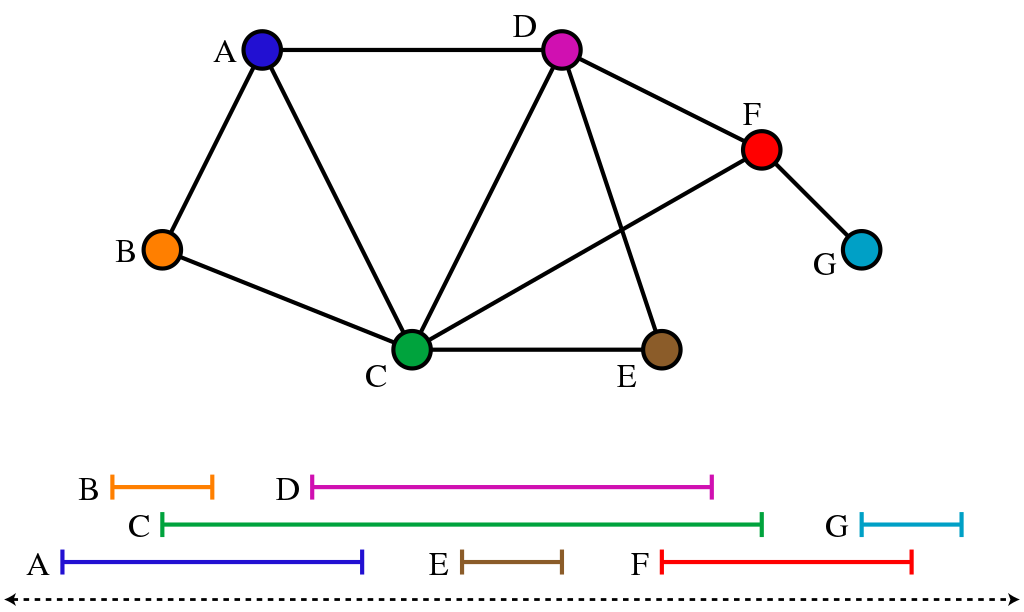
\includegraphics[scale = .3]{4/exercise/intervalgraph.png}
        \caption{Source: Wikipedia}
        \label{fig:my_label}
    \end{figure}

    For a set of intervals $\{I_1, \dots, I_n\}$ with $I_i = (a_i, b_i)$ we sort the endpoints in ascending order to get values $c_1,\dots, c_{2n}$. Consider now the elementary intervals $p_1 := [c_1,c_1], p_2 := (c_1,c_2), p_3 := [c2, c_2], p_4 := (c_2, c_3), \dots$. Now define the path decomposition $T = \{p_i, i\in I\}, \chi: T\to \mathcal P(T), \chi(p_i) = \{I_j\in \{I_1,\dots, I_n\}: I_j\cap p_i\neq \emptyset\}$. Then the axioms for a path decomposition hold:\begin{enumerate}
        \item $\cup_{p\in T\}\chi(t) = V$ as surely every interval $I_i$ must cross one elementary interval.
        \item Let there be an edge $I_iI_j$ in $G$. Then $I_i\cap I_j \neq \emptyset$ and there is an elementary interval $p_k$ that is contained in this intersection, so $I_i, I_j\in \chi(p_k)$.
        \item since the $p_j$ are sorted ascending by their elementary interval, all $p_j's$ containing an interval $I$ are consecutive.
    \end{enumerate}
Now for a $(k+1)$-clique, $k+1$ intverals are all intersecting at a real number $r$ at the same time. In the bag of the elementary interval that contains this $r$, there are thus $k+1$ nodes. There also cannot be a node with more than $k+1$ intervals in it, as that would lead to a clique of more than $k+1$ intervals. Thus :\begin{equation*}
    \mathbf{tw} \leq \text{maximal size of a node} -1 \leq k+1-1 = k
\end{equation*}
\end{solving}
\newpage

%done
\begin{exercise}[Cliques and Tree Decompositions]
    Let $G$ be a graph and $(T,\chi)$ be a tree decomposition of $G$. Prove that, for any clique $W\subseteq V$ of $G$, there must be a node $t\in T$ such that $W\subseteq \chi(t)$.
\end{exercise}
\begin{solving}
    Induction by the size of a clique.
    \begin{enumerate}
        \item[$k= 2$]: A clique of two vertices is just two vertices connected by an edge. By property 2. of the definition of tree decomposition\footnote{ For each $vw\in E$ there is a $t\in V'$ with $v,w\in \chi(t)$}  there has to be a bag of $T$ containing $v$ and $w$.
        \item[$k\to k+1$] A clique $W$ of size $k+1$ contains a subgraph that's a clique $W'$ of size $k$. By the induction hypothesis, there exists a bag $\chi(t)$ containing $W'$. Since $\{v\} = W\backslash W'$ is adjacent to all $v'\in W'$, for all $v'\in W'$ by property 2. of the definition of tree decomposition there is a $t_{v'}$ with $v\in \chi(t_{v'}), v'\in \chi (t_{v'})$\\
        Choose now $v', v'' \in W'$ distinct. Then $t'$ is a children of $t$, so is $t''$, as they each contain $v'$ or $v''$ respectively. As they both contain $v$ however, they must also be connected by property 3. of the definition of the tree decomposition\footnote{For all $v\in V$, $T[\{t\in V'| v\in \chi(t)\}]$ is a connected subtree} and thus the subtree must go through $t$ (otherwise there would be a cycle in the tree generated by $t$. Thus $v\in\chi (t)$.
    \end{enumerate}
\end{solving}
\newpage

% done
\begin{exercise}[Treewidth of Grids]
    Show that the treewidth of the $k\times k$ grid $\mathcal Q_k$ is at least $k$ by describing a winning strategy for the robber against $k$ cops and robber game played on $\mathcal Q_k$.
\end{exercise}
\begin{solving}
    The treewidth is the minimum $k$ such that $k+1$ cops have a strategy to catch a robber in $G$. We thus need to show that the robber can always escape against $k$ cops on the grid.. We lead this by induction in $k$.\\
    For $k=1$ the robber is never placed and is thus never caught. For $k=2$, he can trivially never be caught, as each vertex has two neighbors, of which only ever one is settled by a cop if there is one cop out to catch the robber. The robber is thus always free to move. For $k= 3$, by staying at the side-points of the square, $(0,1), (1,2), (2,1), (1,0)$, as they all have three neighbors that will never be all settled if one cop is moving.\\
    For $k=4$, the robber can always stay in the center square except if all cops are there, but then none of them is moving and cannot catch him. If he is in one of the center squares, he sits on a square with 4 neighbors and cannot be caught.\\
    Assume now that for $k\geq 4$ we know that the robber wins on a $k\times k$ grid with $k$ robbers and can always stay in the center $(k-2)\times(k-2)$-square. Now look at the $(k+1)\times (k+1)$-grid. Assume in the beginning $k+1$ cops are placed. Then, there is a $k\times k$ subgrid, in which there are only $k$ cops (by pigeon hole principle). If the $k+1$st cop does not move, the robber can by assumption still move freely on the $k\times k$-subgrid without losing, even staying in the $(k-1)\times(k-1)$ center subgrid. If the $k+1$st cop does move, he either targets a place outside the current $k\times k$ subgrid with $k$ cops in it, in which case the robber can just keep playing the $k$-cop game in the subgrid, or he targets a place inside of the subgrid, but then there is another $k\times k$ subgrid in which there will be at most $k$ cops and to which the robber may move (even keep in the $(k-2)\times (k-2)$ center) as he kept in the center of the grid.\\
    Thus by induction the robber can always win against $k$ cops.
\end{solving}

\end{document} 